\documentclass[utf8,zihao=-4]{ctexbeamer}
%\documentclass[utf8,zihao=-4,handout,smaller,aspectratio=1610]{ctexbeamer}
\usepackage{multimedia}
\usepackage{hyperref}
\usepackage{smartdiagram}
\usepackage{listings}
\usepackage{tikz}
\usetikzlibrary{shapes.geometric,calc}
\usesmartdiagramlibrary{additions} 
\setbeamercovered{highly dynamic}

%% 所要粘贴代码的编程语言
%\lstloadlanguages{}

%% 设置listings宏包的一些全局样式
%% 参考http://hi.baidu.com/shawpinlee/blog/item/9ec431cbae28e41cbe09e6e4.html
\lstset{
	showstringspaces=false, %设定是否显示代码之间的空格符号
	numbers=left,% 在左边显示行号
	numberstyle=\tiny, % 设定行号字体的大小
	basicstyle=\footnotesize,% 设定字体大小\tiny, \small, \large等等
	keywordstyle=\color{blue!70}, commentstyle=\color{red!50!green!50!blue!50},% 关键字高亮
	frame=shadowbox, % 给代码加框
	rulesepcolor=\color{red!20!green!20!blue!20},
	escapechar=`, % 中文逃逸字符,用于中英混排
	xleftmargin=2em,xrightmargin=2em, aboveskip=1em,
	breaklines,% 这条命令可以让latex自动将长的代码行换行排版
	extendedchars=false % 这一条命令可以解决代码跨页时,章节标题,页眉等汉字不显示的问题
}

\usetheme{madrid}
%\useoutertheme{miniframes}

\usecolortheme{orchid}
\title{ 孔加工概述~~说课}
\author{高星}
\institute{湖南潇湘技师学院~湖南九嶷职院}
\date{2017.12.1}
\begin{document}
    
\begin{frame}[plain]
	\maketitle
	\noindent
    
	\centering	\begin{tabular}[t]{*{4}{l@{~ }}}
			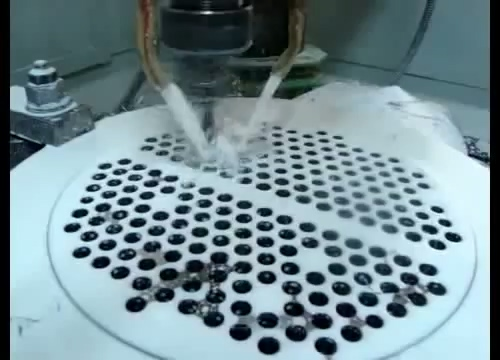
\includegraphics[width=0.22\linewidth,trim=0 0 0 0,clip,angle=0]{image/1.jpg} & 
			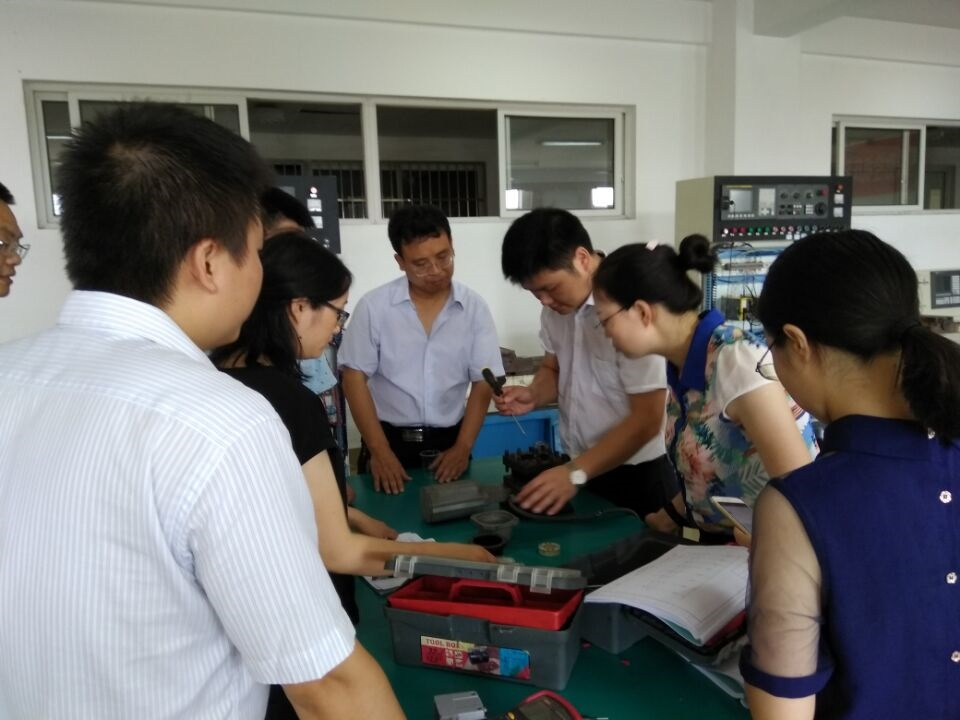
\includegraphics[width=0.22\linewidth,trim=300 1.5cm 0 7cm,clip,angle=0]{image/2.jpg}&
			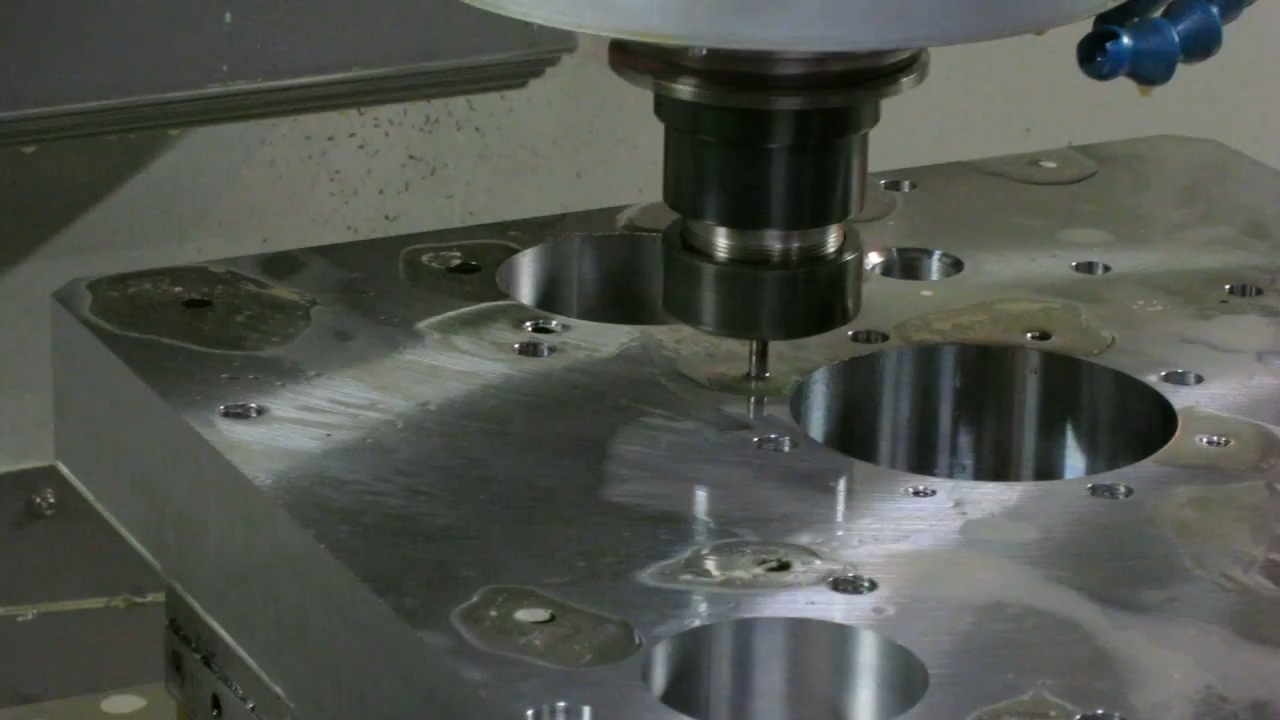
\includegraphics[width=0.22\linewidth,trim=10cm 0 0 0,clip,angle=0]{image/3.jpg}&
			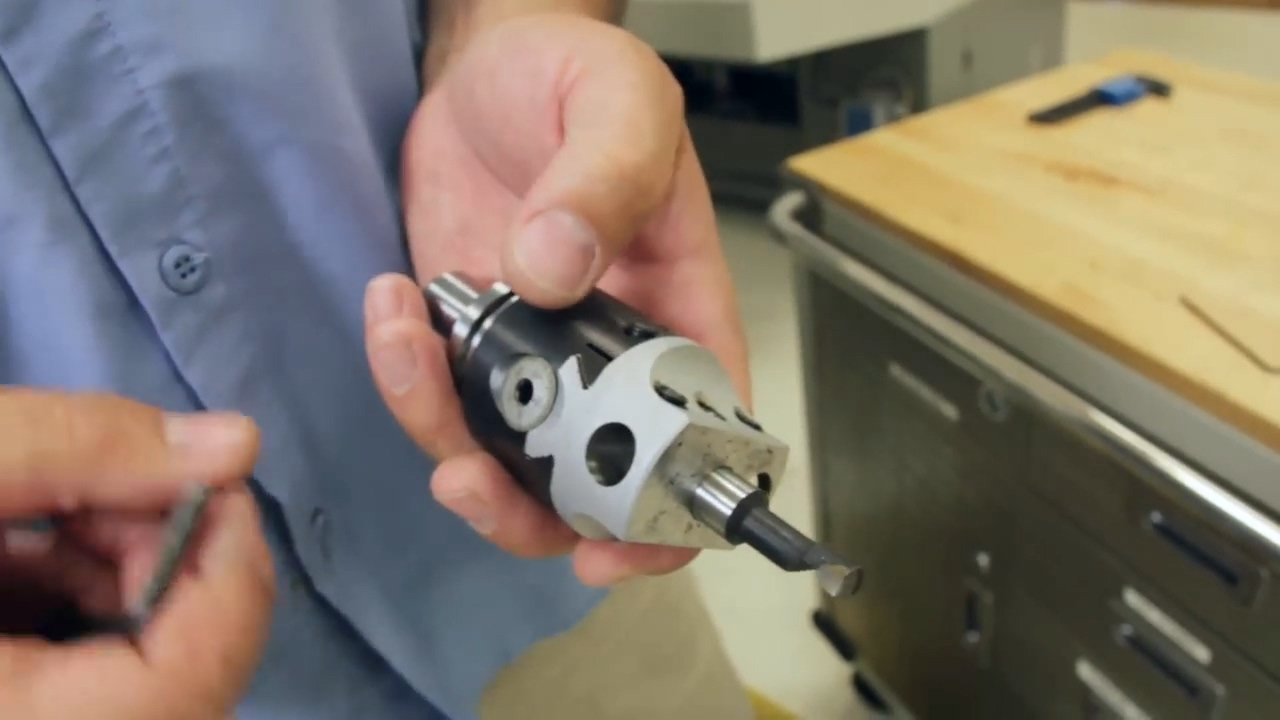
\includegraphics[width=0.22\linewidth,trim=10cm 0  0 0,clip,angle=0]{image/4.jpg}
	\end{tabular}
\vfill 

\end{frame}

\begin{frame}{说课内容}
\begin{columns}[onlytextwidth]

\column[c]{0.1\textwidth}
	
\column[c]{0.3\textwidth}
\tableofcontents[hideallsubsections]

\column[c]{0.6\textwidth}
\vspace{0.5cm}

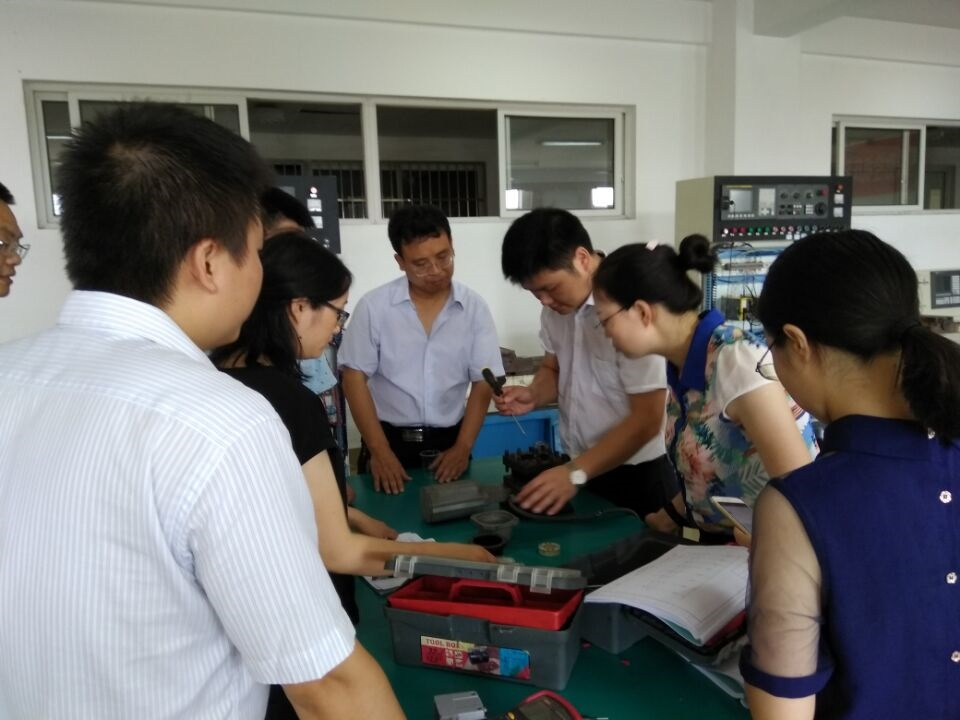
\includegraphics[width=0.9\linewidth,trim=0 0 0 0,clip,angle=0]{image/2.jpg}
\end{columns}

\end{frame}

\section{说教材}
\subsection{教材选择}
\begin{frame}{教材选择}
	\begin{columns}[onlytextwidth]
		\column{.5\textwidth}

\begin{enumerate}
   \item<1-> 教材:《数控机床编程与操作(数控铣床/加工中心分册)》,中国劳动出版社,沈建峰     
     
\end{enumerate}
    \onslide<2-> 
\smartdiagramset{border color=black,%边界颜色
   	set color list={blue!50!cyan,green!60!lime,orange!50!red,red!80!black},%颜色列表
    module x sep=5cm,%向间距
    module y sep=1.5cm,%向间距
    uniform arrow color=true,%是否制定颜色
    arrow color=white,%箭头颜色
    arrow line width=0.5cm,%箭头宽度
   	back arrow disabled=true,%是否箭头返回
%   module minimum width=5cm,%最小宽度
%module minimum height=2cm,%最小高度
text width=4cm,%文本宽度
}
  \begin{center}
       \smartdiagram[flow diagram]{出版社重视技能,与本学校系统相同}
  \end{center}     

	\column{.5\textwidth}
    \onslide<1->
\includegraphics[width=0.9\linewidth,trim=0 0 0 0,clip,angle=0]{image/5.jpg}
	\end{columns}
\end{frame}

\begin{frame}{参考书}
	 \begin{itemize}
	 	\item<1->《国家职业标准----加工中心操作工》,劳动社会保障出版社
	 	\item<2->《加工中心编程与操作》,科学出版社,主编刘加孝 
	 	\item<3->《数控铣削宏程序及应用实例》,机械工业出版社,陈海舟
	 	\item<4-> 《fanuc 编程说明书》、《数控加工工艺》

	 	
	 \end{itemize}
% \centering
 \hspace{2cm}\includegraphics<1->[width=0.22\linewidth,trim=0 0 0 0,clip,angle=0]{image/7.jpg}~~ 
 \includegraphics<2->[width=0.22\linewidth,trim=0 0 0  0,clip,angle=0]{image/6.jpg}~~
\includegraphics<3->[width=0.22\linewidth,trim=0 0 0 0,clip,angle=0]{image/8.jpg} 
 
\end{frame}






\subsection{教材中的位置与地位}
\begin{frame}{教材中的位置与地位}
 	\begin{columns}[onlytextwidth]
 	\column{.4\textwidth}
 	 \begin{itemize}
 		\item<1->《国家职业标准---加工中心操作》手工编程必考内容
 		
 		\item<2->比赛手工编程四大结构之一
 		
 		\item<3-> 教材第二章第三节、第四章第三节
	\end{itemize}
 	\column{.6\textwidth}
\begin{center}
\smartdiagramset{border color=black,%边界颜色
    set color list={blue!50!cyan,green!60!lime,orange!50!red,red!80!black,blue!50!cyan,green!60!lime,orange!50!red,red!80!black},%颜色列表
    module x sep=5cm,%向间距
    module y sep=1.5cm,%向间距
    uniform arrow color=true,%是否制定颜色
    arrow color=white,%箭头颜色
    arrow line width=0.5cm,%箭头宽度
    back arrow disabled=true,%是否箭头返回
    %   module minimum width=5cm,%最小宽度
    %module minimum height=2cm,%最小高度
    text width=8cm,%文本宽度
    bubble fill opacity=0
}
\scalebox{0.7}{
\smartdiagram[connected constellation diagram]{数控铣编\\程与操作,基本知识,平面加工,外形加工,挖槽加工,孔加工,简化编程}%中心主题
}

\end{center}

	\end{columns}    
\end{frame}

\subsection{主题安排}
\begin{frame}{主题安排}
    
    \begin{center}
        \smartdiagramset{border color=black,%边界颜色
            set color list={blue!50!cyan,green!60!lime,orange!50!red,red!80!black,blue!50!cyan,green!60!lime,orange!50!red,red!80!black},%颜色列表
            module x sep=5cm,%向间距
            module y sep=1.5cm,%向间距
            uniform arrow color=true,%是否制定颜色
            arrow color=white,%箭头颜色
            arrow line width=0.5cm,%箭头宽度
            back arrow disabled=true,%是否箭头返回
            %   module minimum width=5cm,%最小宽度
            %module minimum height=2cm,%最小高度
            text width=8cm,%文本宽度
            bubble fill opacity=0
        }
        \scalebox{0.7}{
            \smartdiagram[connected constellation diagram]{孔加工,孔加工概述,Fanuc孔加工编程及工艺,fanuc孔加工详解,Siemen孔加工编程,仿真及机床操作}%中心主题
        }
\end{center}
\end{frame}

\subsection{主题分析}
\begin{frame}{主题分析}
	\begin{columns}[onlytextwidth]
	\column{.1\textwidth}
	\column{.8\textwidth}
	\begin{itemize}
		\item<1-> 前面学习了挖槽加工,其中有圆形槽加工。
		\item<2-> 后面要学Fanuc、Siemens孔加工固定循环。
		\item<3-> 孔加概述承前启后主要为后面的学习打基础。
		
		
	\end{itemize}
   \vspace{0.5cm}
	\includegraphics<1->[width=0.33\linewidth,trim=400 300 600 400,clip,angle=0]{image/9.jpg}~~ 
	\includegraphics<2->[width=0.33\linewidth,trim=0 0 0  0,clip,angle=0]{image/1.jpg}~~
	\includegraphics<3->[width=0.33\linewidth,trim=10cm 0 0 0,clip,angle=0]{image/3.jpg}
	\column{.1\textwidth}
	 \end{columns}
\end{frame}

\subsection{教学目标}
\begin{frame}{教学目标}
 \begin{columns}[onlytextwidth]
    \column{.15\textwidth}
    \column{.7\textwidth}
    \begin{block}{知识目标}
        \begin{enumerate}[<+->]
            \item 掌握孔加工的方式;
            \item 掌握传统孔加工的刀具;
            \item 了解铣孔与传统孔加工的区别;
            \item 掌握孔加工的6个动作与3个平面;
            \item 能结合子程序编写孔加工程序;
        \end{enumerate}
    \end{block}
    \column{.15\textwidth}
 \end{columns}
\end{frame}

\begin{frame}{教学目标}
	\begin{columns}[onlytextwidth]
		\column{.15\textwidth}
		\column{.7\textwidth}
		\begin{block}{能力目标}
			\begin{enumerate}[<+->]
				\item ;
				\item 掌握传统孔加工的刀具;
				\item 了解铣孔与传统孔加工的区别;
				\item 掌握孔加工的6个动作与3个平面;
				\item 能结合子程序编写孔加工程序;
			\end{enumerate}
		\end{block}
		\column{.15\textwidth}
	\end{columns}
\end{frame}

\subsection{重点难点}
\begin{frame}{重点难点}
 \begin{columns}[onlytextwidth]
	\column{.2\textwidth}
	\column{.6\textwidth}
	\begin{block}{重点难点}
		\begin{enumerate}[<+->]
			\item 掌握孔加工的方式;
			\item 掌握传统孔加工的刀具;
			\item 了解铣孔与传统孔加工的区别;
			\item 掌握孔加工的6个动作与3个平面;
			\item 能结合子程序编写孔加工程序;
		\end{enumerate}
	\end{block}
	\column{.2\textwidth}
\end{columns}
\end{frame}


\section{说教法}
\begin{frame}{案例分析}
     \begin{columns}[onlytextwidth]
        \column{.4\textwidth}
        在数控铣床或加工中心上加工如图所示的零件,试完成程序的编写,已知毛坯为 $\phi$ 110*30。
        \column{.6\textwidth}

\begin{figure}
    \centering
    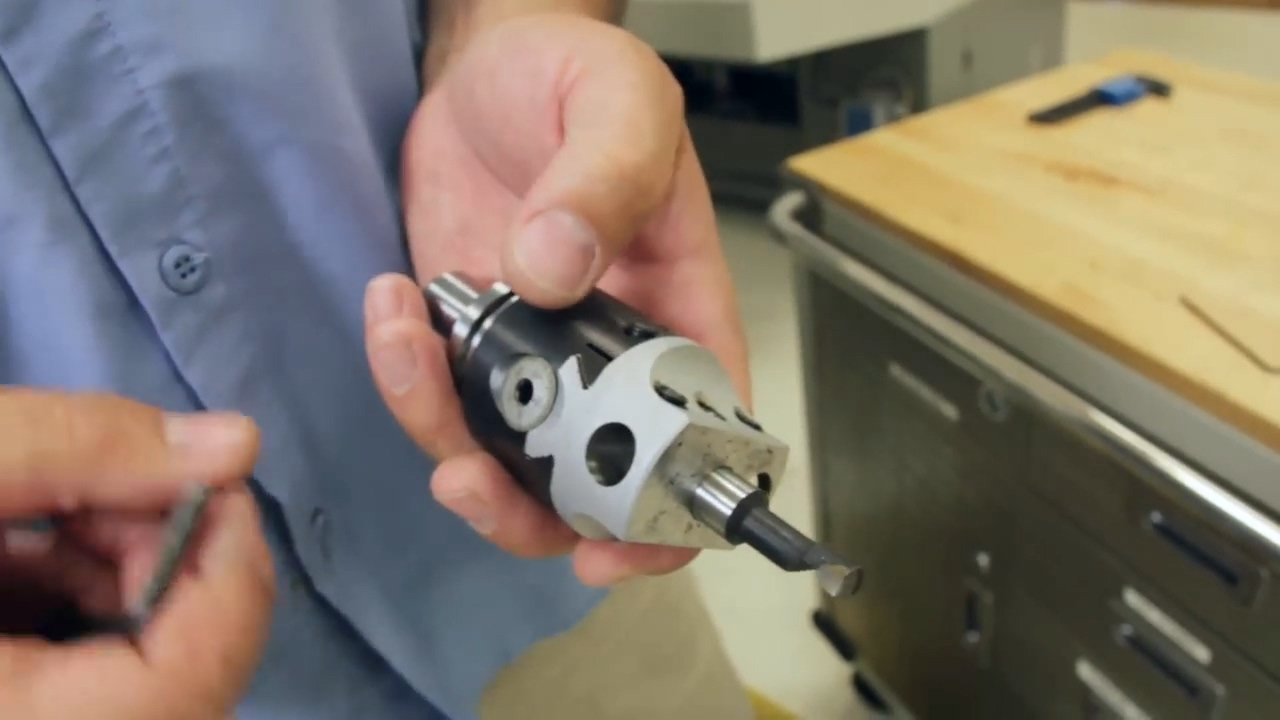
\includegraphics[width=0.8\linewidth,trim=50 150 50 100,clip]{image/4.jpg}
%    \caption{}
    \label{fig:4-1}
\end{figure}
    \end{columns}
\end{frame}

\begin{frame}{手工编程流程}
    \begin{columns}[onlytextwidth]
        \column{.2\textwidth}
        \column{.8\textwidth}
\begin{enumerate}
    \item 图样分析;
    \item 确定加工内容;
    \item 确定装夹及工件坐标系;
    \item 确定刀具及切削用量;
    \item 确定工序及走刀路线;
    \item 计算点坐标;
    \item 编写程序单。
\end{enumerate}
    \end{columns}
\end{frame}


\section{说学法}
\begin{frame}{g0与g1的区别}
    \begin{columns}[onlytextwidth]
        \column{.0\textwidth}
        \column{\textwidth}
\begin{enumerate}
    \item 指令格式不同:g1使用前必须用f设定进给速度,g0的速度与f无关 
    \item 运动轨迹不同:g0为快速定位,其路径可能为直线,也可能为折线。g1为直线插补,其路径为直线。
    \item 进给速度不同:g0的速度由机床参数及快速倍率决定,档位少。g1的速度由f及进给倍率决定,可调档位多。
    \item 功能用途不同:g0用于加工前的定位及加工后的提刀,g1用于车削加工
\end{enumerate}
    \end{columns}
\end{frame}


\begin{frame}{怎样确定一个圆弧}
    \begin{columns}
        \column{.3\textwidth}
        \column{\textwidth}
    \end{columns}
\end{frame}

\begin{frame}{怎样确定一个圆弧}
    \begin{columns}
        \column{.3\textwidth}
        \column{\textwidth}
        \begin{enumerate}
            \item 圆弧三点
            \item 起点、终点、圆心
            \item 2点半径
            \item 圆心、半径、起始角、终止角
            \item 其他
        \end{enumerate}
    \end{columns}
\end{frame}

\begin{frame}{数控机床圆弧编程}
    \begin{columns}
        \column{.2\textwidth}
        \column{0.6\textwidth}
        \begin{enumerate}
            \item 圆弧编程 (r)
            \item 圆心编程 (ijk)
        \end{enumerate}
         \vspace{1cm}
         圆心编程 (ijk)为标准格式,自动编程常用,手工编程一般用于整圆。
         
         圆弧编程 (r),指令符合图样标注,使用较多。
         \column{.2\textwidth}
    \end{columns}
\end{frame}

\begin{frame}{圆弧编程格式}
    \begin{columns}
        \column{0.6\textwidth}

 \begin{enumerate}
     \item xy平面的圆弧 
   
 g17  g2/g3  g90/g91 x\_ y\_ r\_ f\_
 
 \item zx平面的圆弧 
   
 g18 g2/g3 g90/g91 z\_ x\_ r\_ f\_
 
\item  yz平面的圆弧   
 
 g19 g2/g3 g90/g91 y\_ z\_ r\_ f\_
 
 \end{enumerate}
  对于我们学校的一般用g17平面
        \column{.4\textwidth}
        \begin{figure}
            \centering
            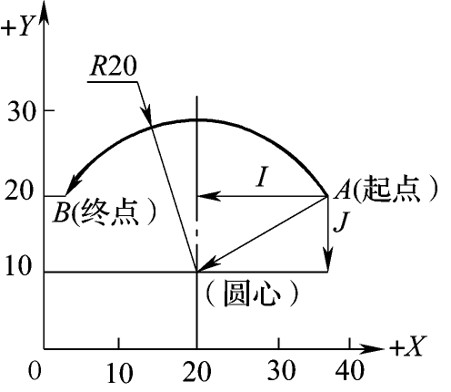
\includegraphics[width=1\linewidth]{image/4-3}
            \caption{}
            \label{fig:4-3}
        \end{figure}
        
        
    \end{columns}
\end{frame}


\begin{frame}{圆弧编程格式}
    \begin{columns}
        \column{.1\textwidth}
        \column{0.8\textwidth}
        
      指令格式的说明
      
      g17	指定圆弧在xpyp平面
      
      g18	指定圆弧在xpzp平面
      
      g19	指定圆弧在ypzp平面
      
      g02	顺时针方向圆弧插补(cw)
      
      g03	逆时针方向圆弧插补(ccw)
      
      x\_\_	终点的x坐标
      
      y\_\_	终点的y坐标
      
      z\_\_	终点的z坐标
      
      r\_\_	圆弧半径指定的带符号的圆弧半径
      
      f\_\_	沿圆弧的进给率           
        
        \column{.1\textwidth}
    \end{columns}
\end{frame}



\begin{frame}{圆弧插补的方向}
    \begin{columns}

        \column{0.6\textwidth}
g2:顺时针方向:左上右 (拧紧水平盖)

g3:逆时针方向:右上左

在数学上,规定顺时针旋转的角为负角,逆时针旋转的角为正角。


观察点:从第三轴的正方向向负方向看。


        \column{.4\textwidth}
        
        \begin{figure}
            \centering
            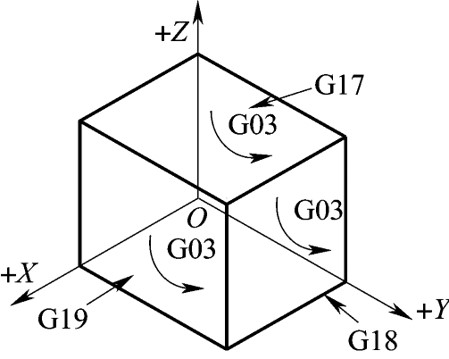
\includegraphics[width=\linewidth]{image/4-2}
            \caption{}
            \label{fig:4-2}
        \end{figure}
        
\end{columns}
\end{frame}


\begin{frame}{举例}
\begin{figure}
    \centering
    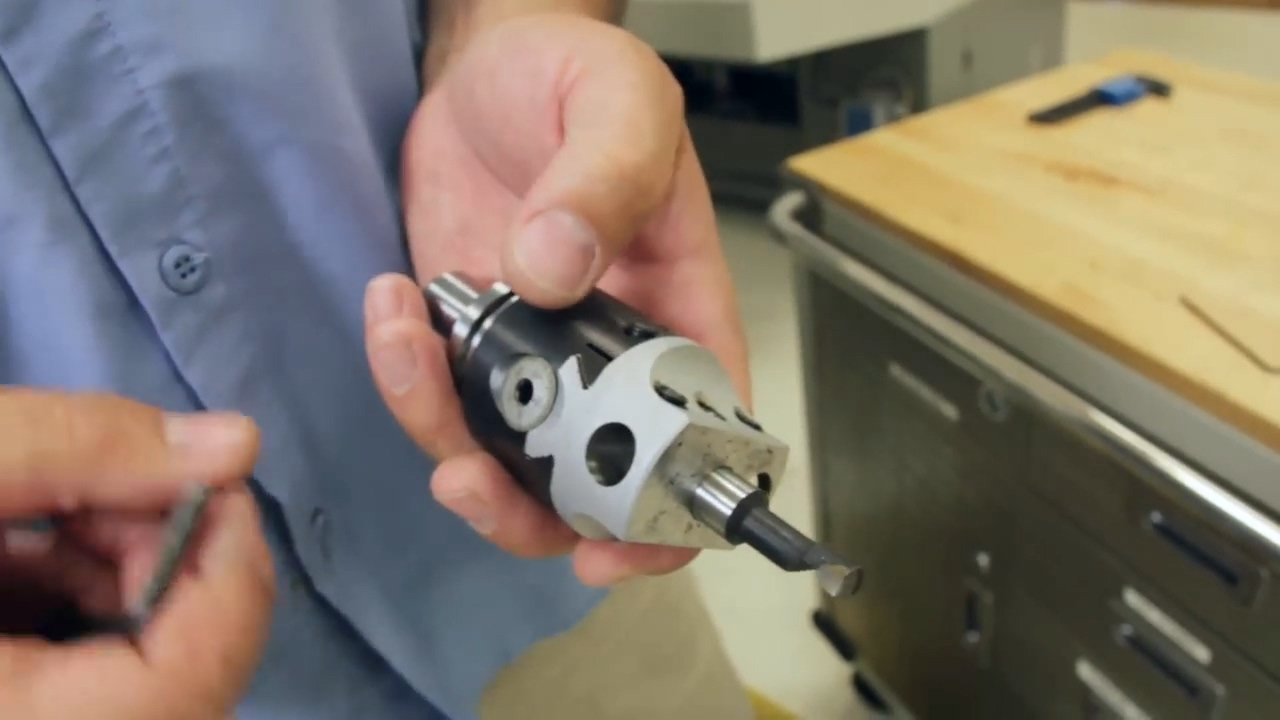
\includegraphics[width=0.5\linewidth,trim=50 150 50 100,clip]{image/4.jpg}
    %    \caption{}
    \label{fig:4-7}
\end{figure}        
\end{frame}

\begin{frame}{g91/g90}
 \begin{figure}
     \centering
     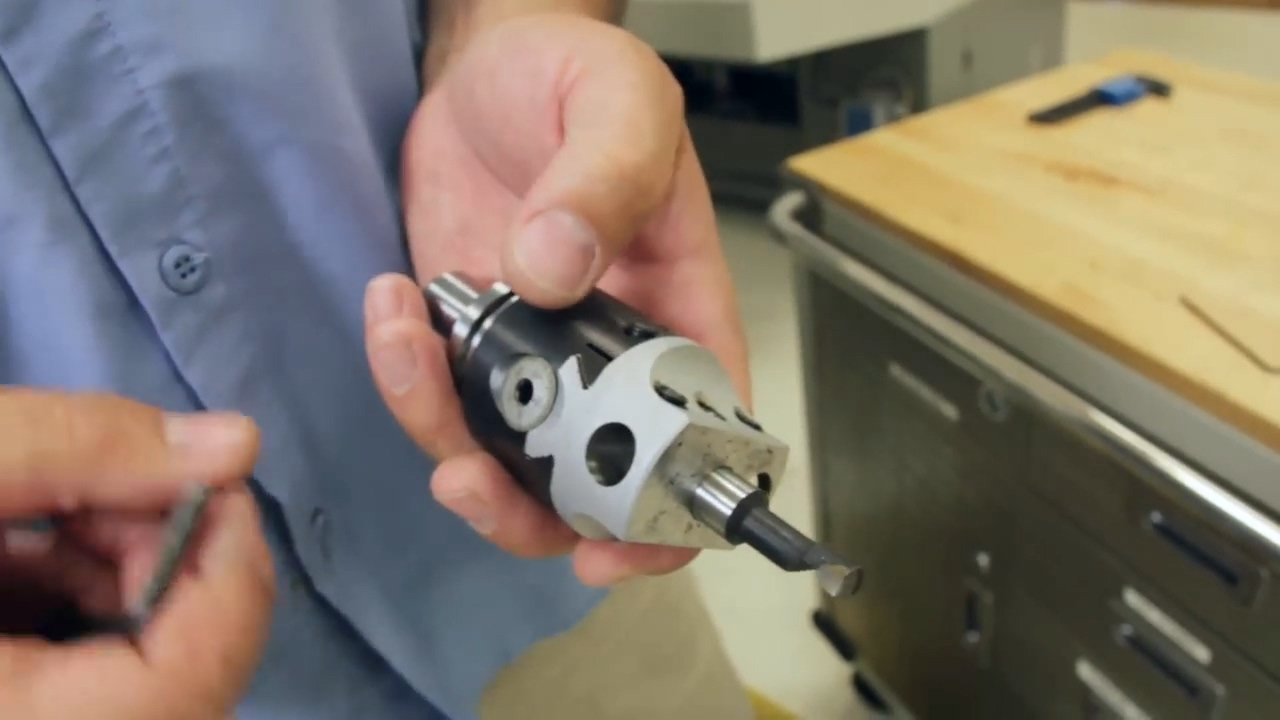
\includegraphics[width=0.5\linewidth,trim=50 150 50 100,clip]{image/4.jpg}
     %    \caption{}
     \label{fig:4-8}
 \end{figure}       
\end{frame}


\AtBeginSection{
	\begin{frame}{提纲}
		\tableofcontents[currentsection,hideallsubsections]
	\end{frame}
}
\AtBeginSection{
	\begin{frame}{提纲}
		\tableofcontents[currentsection,currentsubsection]
	\end{frame}
}


\section{说教学过程}
\AtBeginSection{
\begin{frame}{圆弧凸台编程实例}
    \begin{figure}
        \centering
        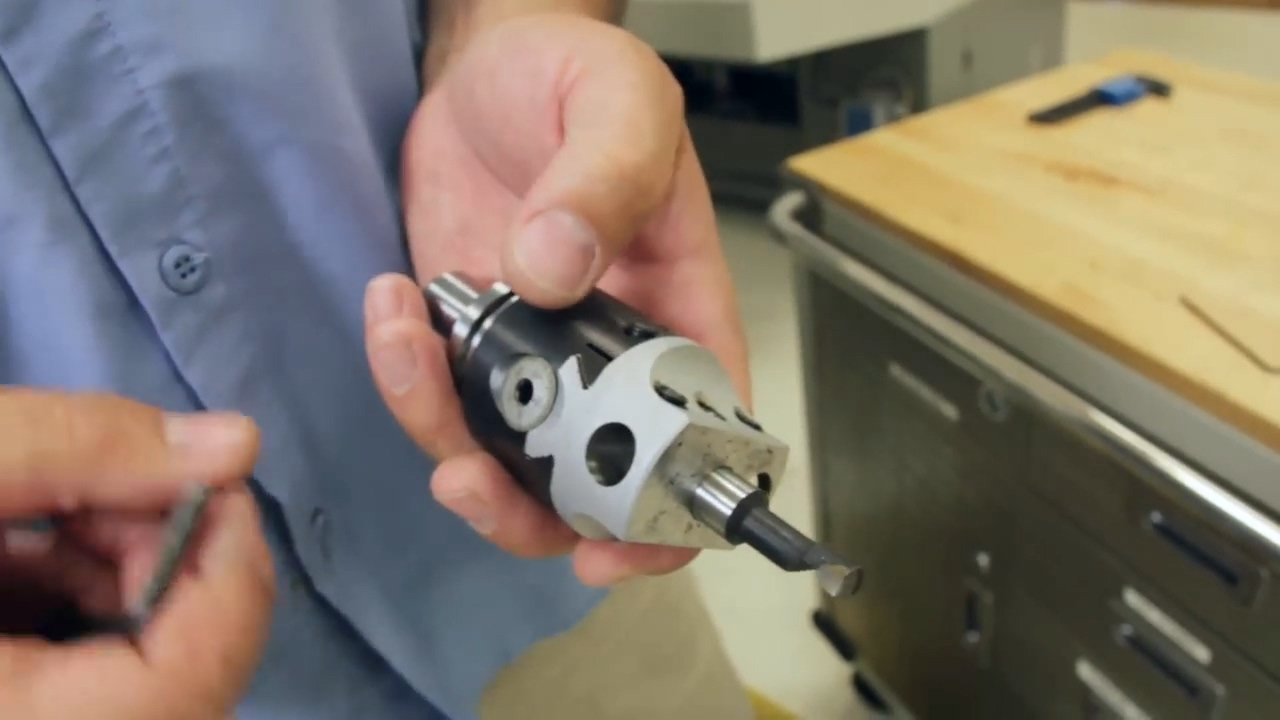
\includegraphics[width=0.5\linewidth,trim=50 150 50 100,clip]{image/4.jpg}
        %    \caption{}
        \label{fig:4-8}
    \end{figure}       
\end{frame}
}

\section{说教学反思}
\begin{frame}{零件编程}
    \begin{columns}
        \column{.0\textwidth}
        \column{\textwidth}
 程序初始化(安全保护)--------辅助准备(换刀,主轴启动,切削液开)--------定位到起刀点--------快速下刀--------工进下刀--------走加工轮廓--------提刀---------快速提刀到安全平面-------程序结束(换刀,主轴停止,切削液关,程序返回等)       
        
    \end{columns}
\end{frame}



\section*{课堂小结}
\begin{frame}{课堂小结}

    \begin{columns}
        \column{.2\textwidth}
        \column{.8\textwidth}
\begin{enumerate}[<+-> ]
\item g1与g0的区别。
\item 圆弧指令的两种方式。
\item 半径编程的格式。
\item 方向的判断。
\item 指令的使用。
\item 编写程序的基本思路
\end{enumerate}
    \end{columns}
\end{frame}

\begin{frame}{作业}
\begin{enumerate}
    \item 自定尺寸,编写加工一个圆弧凸台的数控程序。
\end{enumerate}
\end{frame}

\begin{frame}[plain]
\vfill

\centering \huge 谢谢大家!

\vfill

\flushleft \footnotesize   
~~~qq:32731964\\
~~~tel:18974681118\\
%~~~课件下载:\\
%~~~https://github.com/gnixoag/myworks2017/tree/master/jiaoshichengzhang

\end{frame}

\section*{模板设计}
\begin{frame}{模板设计}
    \begin{center}
        \smartdiagramset{border color=black,%边界颜色
            set color list={blue!50!cyan,green!60!lime,orange!50!red,red!80!black},%颜色列表
            module x sep=5cm,%向间距
            module y sep=1.5cm,%向间距
            uniform arrow color=true,%是否制定颜色
            arrow color=white,%箭头颜色
            arrow line width=0.5cm,%箭头宽度
            back arrow disabled=true,%是否箭头返回
            %   module minimum width=5cm,%最小宽度
            %module minimum height=2cm,%最小高度
            text width=4cm,%文本宽度
        }
        %\smartdiagram[circular diagram]{一,二,三,四,五}%圆形,逆时针。
        %\smartdiagram[circular diagram:clockwise]{一,二,三,四,五}%圆形,顺时针。
        %\smartdiagram[flow diagram]{一,二,三,四,五}%垂直流线。
        %\smartdiagram[flow diagram:horizontal]{一,二,三,四,五}%水平流线。
        %\smartdiagram[descriptive diagram]{{一,{一一}},{二,{二二}},{三,{三三}},{四,{四四}},{五,{五五}}}%详细
        %\smartdiagram[priority descriptive diagram]{一,二,三,四,五}%层次详细
        \smartdiagram[bubble diagram]{数控铣编程与操作,基本知识,平面加工,外形加工,挖槽加工,孔加工,简化编程}%中心主题
        %\smartdiagram[constellation diagram]{一,二,三,四,五}%中心主题,带箭头。
        %\smartdiagram[connected constellation diagram]{一,二,三,四,五}%中心主题,子项相连。
        %\smartdiagram[sequence diagram]{{一,{一一}},{二,{二二}},{三,{三三}},{四,{四四}},{五,{五五}}}%箭头向前。
    \end{center}
    
\end{frame}

\end{document} 
